%   ____                    _ _ _       ____                                 
%  / __ \                  | | ( )     |  _ \                                
% | |  | |_ ____      _____| | |/ ___  | |_) | ___  __ _ _ __ ___   ___ _ __ 
% | |  | | '__\ \ /\ / / _ \ | | / __| |  _ < / _ \/ _` | '_ ` _ \ / _ \ '__|
% | |__| | |   \ V  V /  __/ | | \__ \ | |_) |  __/ (_| | | | | | |  __/ |   
%  \____/|_|    \_/\_/ \___|_|_| |___/ |____/ \___|\__,_|_| |_| |_|\___|_|   
%                                                                            
%If you have any question,please tell me!
%mail:3013sxc@gmail.com
%github:1anSong

\documentclass[xcolor=table]{beamer}
\usetheme{CambridgeUS}
\useinnertheme{circles}
\useoutertheme{miniframes}
\setbeamertemplate{itemize items}[circle]
\setbeamercolor{itemize item}{fg=red}
\setbeamercolor{itemize/enumerate body}{fg=gray}
\bibliographystyle{plain}
\newtheorem{thm}{定理}
\usepackage{colortbl}
\usepackage{xcolor}
\usepackage{tikz}
\usepackage[UTF8,noindent]{ctexcap}
%==================================================================
\title{杂谈勾股定理}
\subtitle{数学史讲座之一}
\author{Xiangcong Song}
\institute{FUNSOM}
\date{\today}
%\subject{勾股定理}
%\keywords{hello}

\begin{document}
\frame{\titlepage}

\begin{frame}
\tableofcontents	
\end{frame}

\section{勾股定理在古代}
\begin{frame}{古希腊数学}
	勾股定理在西方称为毕达哥拉斯定理,古希腊数学家在2000多年前就已经发现并证明了它$^{\cite{e}}$
	\begin{itemize}
			\item 公元前6世纪,毕达哥拉斯学派发现了一个法则,可以构造直角三角形的边长;
			\item 公元前3世纪,欧几里德《几何原本》使用面积法证明勾股定理。
		\end{itemize}
\end{frame}

\begin{frame}{古中国数学}{定理发现}
中国在3000年前就知道勾股数的概念,比古希腊更早一些。

《周髀算经》的记载:
\begin{itemize}
	\item 公元前11世纪,商高答周公问:
		\begin{quote} 
		勾广三,股修四,径隅五。	
		\end{quote}
	\item 又载公元前 7--6 世纪陈子答荣方问,表述了勾股定理的一般形式:
		\begin{quote}
			若求邪至日者,以天下为勾,日高为股,勾股各自乘,并而开方除之,得邪至日。
		\end{quote}
\end{itemize}
\end{frame}

\begin{frame}
	\frametitle{古中国数学}
	\framesubtitle{定理证明}
	有论者认为早在公元前11世纪商告即已证明勾股定理,完整的证明见于三国(公元前3世纪)赵爽对《周髀算经》的注释。
\end{frame}

\section{勾股定理在现代}
\begin{frame}{现代叙述}{}
	\begin{thm}[勾股定理]
		直角三角形斜边的平方等于两直角边的平方和。

		可以用符号语言表述为:设直角三角形$ABC$,其中
		\begin{equation}
			AB^2=BC^2+AC^2
		\end{equation}
	\begin{center}
		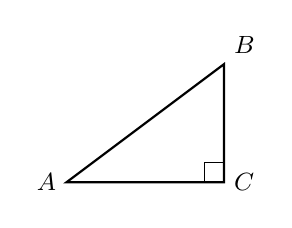
\begin{tikzpicture}[scale=0.5,font=\small]
			\draw[thick] (0,0) node[left] {$A$}
				-- (4,0) node[right] {$C$}
				-- (4,3) node[above right]{$B$} --cycle;
			\draw (3.5,0) |- (4,0.5);
		\end{tikzpicture}
	\end{center}
	\end{thm}
\end{frame}

\begin{frame}
	满足式(1)的整数称为\emph{勾股数}。第一节所说毕达哥拉斯学派得到的三元数组就是勾股数。
	

\rowcolors{2}{gray!25}{gray!50}
	\begin{tabular}{rrr}
		\rowcolor{gray} 直角边 $a$ & 直角边 $b$ & 斜边 $c$\\
		3 & 4 & 5 \\	
		5 & 12 & 13 \\	
		7 & 24 & 25 \\	
		8 & 15 & 17 \\	
	\end{tabular}
\end{frame}


\begin{frame}
\bibliography{math}
\end{frame}

\end{document}
